\section{High-Performance Computing Aspects}
This section examines MFEM's high-performance computing capabilities.

\subsection{Parallel Mesh Processing}
MFEM excels in large-scale parallel computing using MPI. It divides problems into smaller parts for parallel processing. For instance, Figure \ref{fig:2.1} illustrates the parallel solution of a Poisson problem.

% \begin{figure}[H]
%     \centering
%     \hspace{0.75cm}
%     \begin{subfigure}{0.4\textwidth}
%         \includegraphics[width=\textwidth]{Figures/Figure_2_1.png}
%     \end{subfigure}
%     \hfill
%     \begin{subfigure}{0.4\textwidth}
%         \includegraphics[width=\textwidth]{Figures/Figure_2_2.png}
%     \end{subfigure}
%     \hspace{0.75cm}
%     \caption{Left: Solving a Poisson problem in parallel on 100 processors. Right: Unstructured parallel decomposition of a fourth order NURBS mesh of the unit ball on 16 processors.}
%     \label{figure_2}
% \end{figure}

\begin{figure}[H]
    \centering
    \begin{subfigure}[t]{0.45\textwidth}
        \centering
        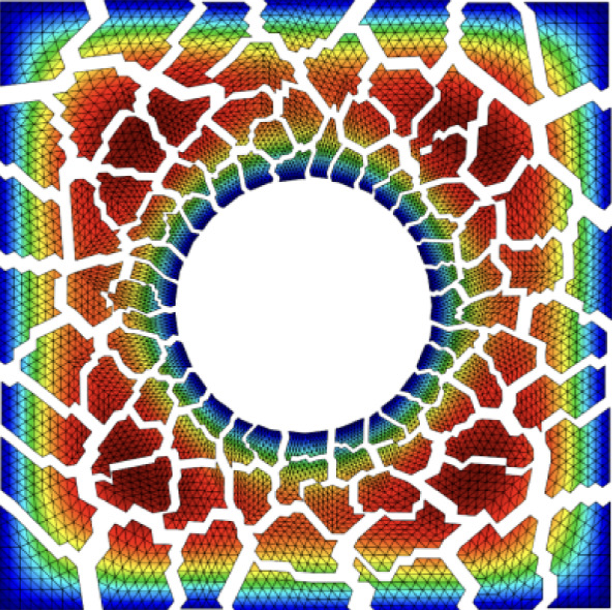
\includegraphics[height=5.5cm,keepaspectratio]{figures/f2_1.png}
        \caption{Solving a Poisson problem in parallel on 100 processors}
        \label{fig:2.1}
    \end{subfigure}
    \hfill
    \begin{subfigure}[t]{0.45\textwidth}
        \centering
        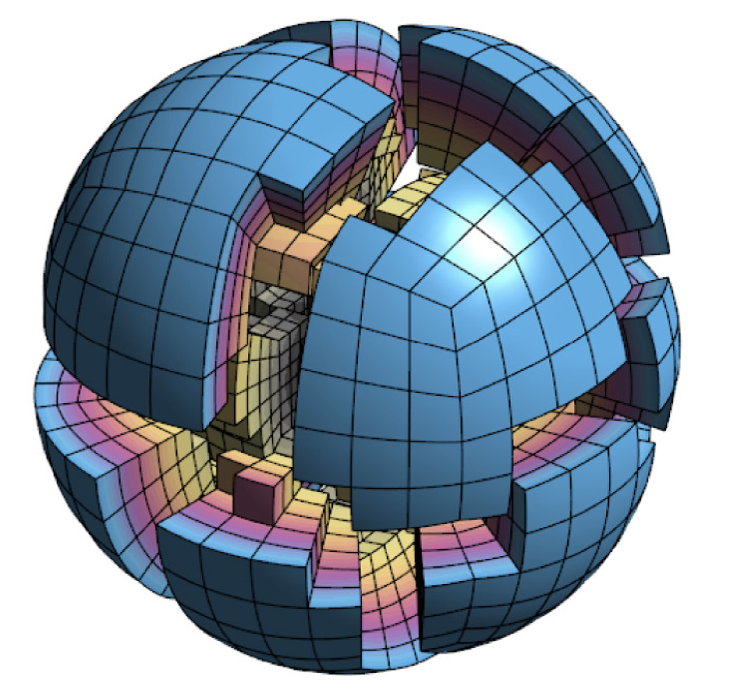
\includegraphics[height=5.5cm,keepaspectratio]{figures/f2_2.png}
        \caption{Unstructured parallel decomposition of a fourth order NURBS mesh of the unit ball on 16 processors}
        \label{fig:2.2}
    \end{subfigure}
    \caption{Illustrations of Parallel Solutions}
    \label{fig:2}
\end{figure}



\subsection{GPU Acceleration}
MFEM 4.0 introduced compatibility with hardware accelerators, enhancing performance with GPUs. It supports various backends for increased efficiency. The structure of the backend selection process is demonsrated in figure \ref{figure_3}

\begin{figure}[H]
    \centering
    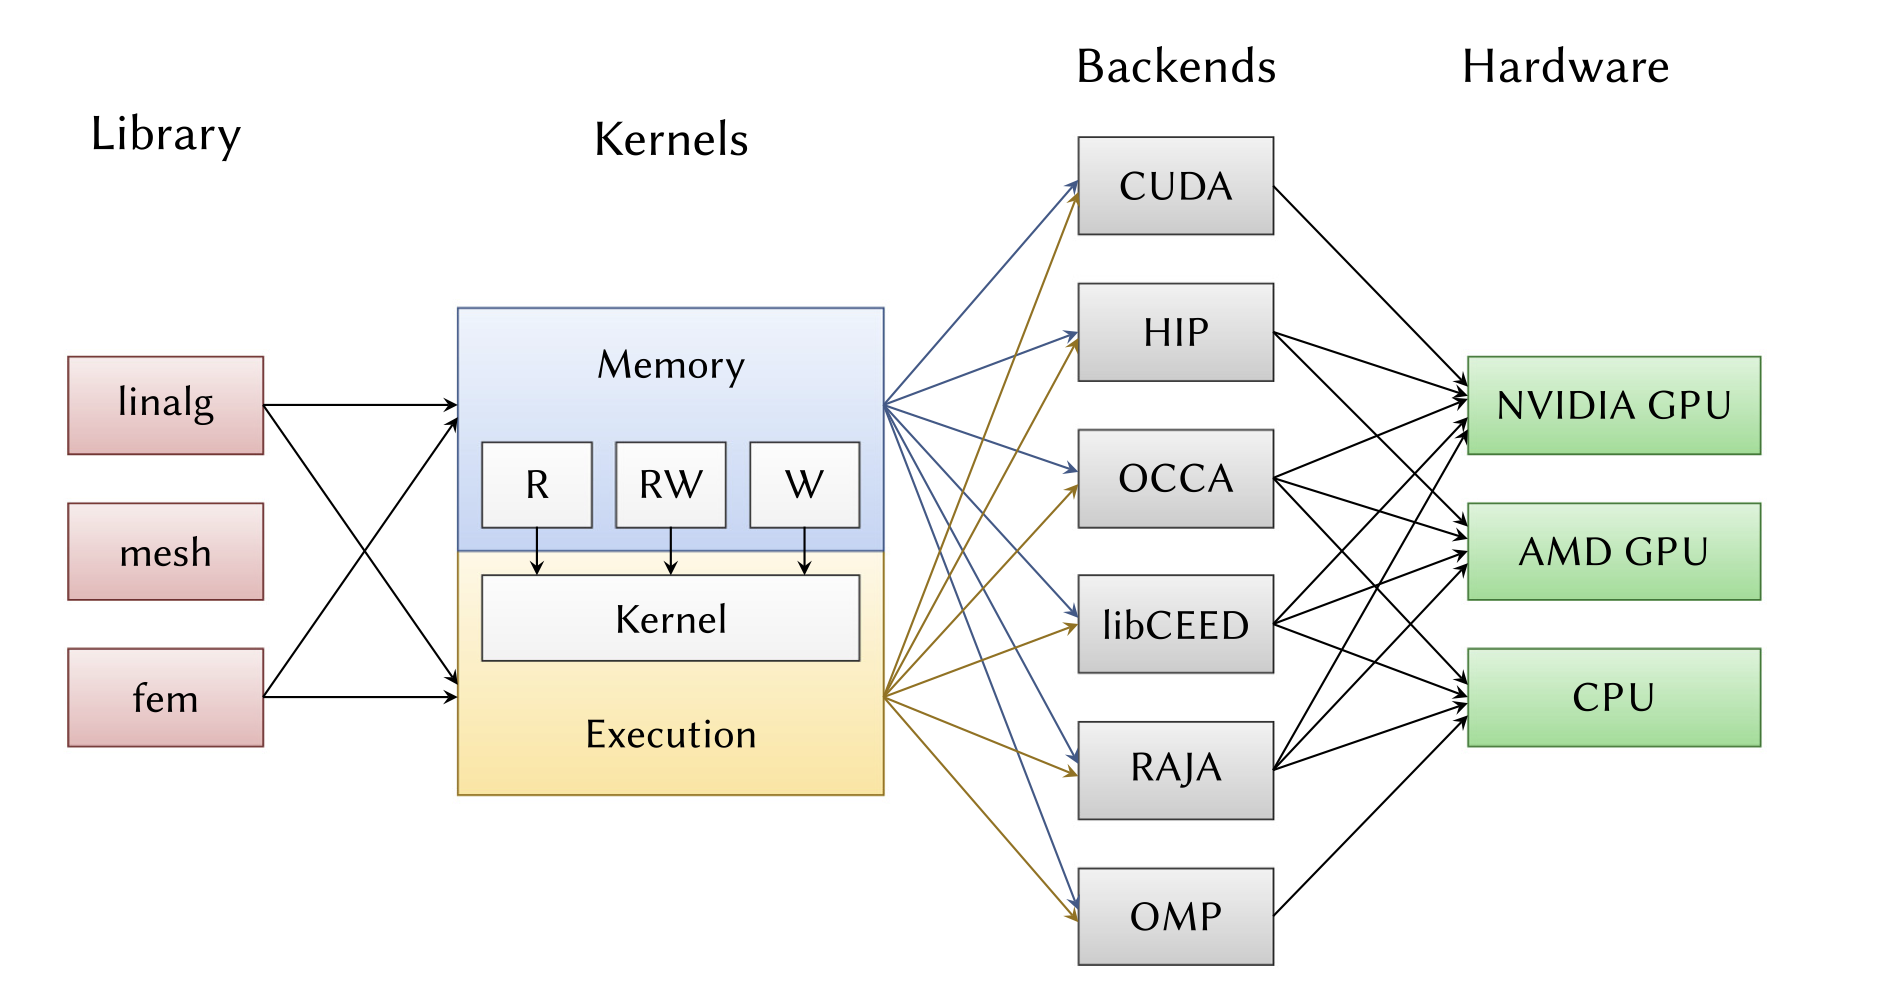
\includegraphics[width=1.0\textwidth]{figures/f3.png}
    \caption{Diagram of MFEM’s modular design for accelerator support. }
    \label{figure_3}
\end{figure}

